%!TEX TS-program = pdflatex
\documentclass[a5paper,12pt,draft]{book}

\usepackage[utf8]{inputenc}
% \usepackage[T1]{fontenc}

\usepackage{charter}
\renewcommand{\rmdefault}{bch}

\usepackage{helvet}
\renewcommand{\sfdefault}{phv}

% \renewcommand{\familydefault}{\sfdefault} % \rmdefault

\usepackage[top=20.0mm, bottom=20.0mm, left=25.0mm, right=20.0mm]{geometry}
\setlength{\marginparwidth}{0.0pt}
\setlength{\footskip}{20.0pt}

% \usepackage{showframe} % DEBUG

\usepackage[final]{graphicx}

\usepackage{hyperref}
\hypersetup{final=true, colorlinks=true}
% \urlstyle{same}

\pagestyle {plain}
\setlength{\parindent}{1.5em}
\setlength{\parskip}{1.0em}


% Book
\begin{document}

% Title page
\begin{titlepage}
\vspace*{\stretch{2}}
\begin{center}
    \textbf{\huge{Croatian chess}} \\
    \large{and other variants} \\ [2.0cm]

    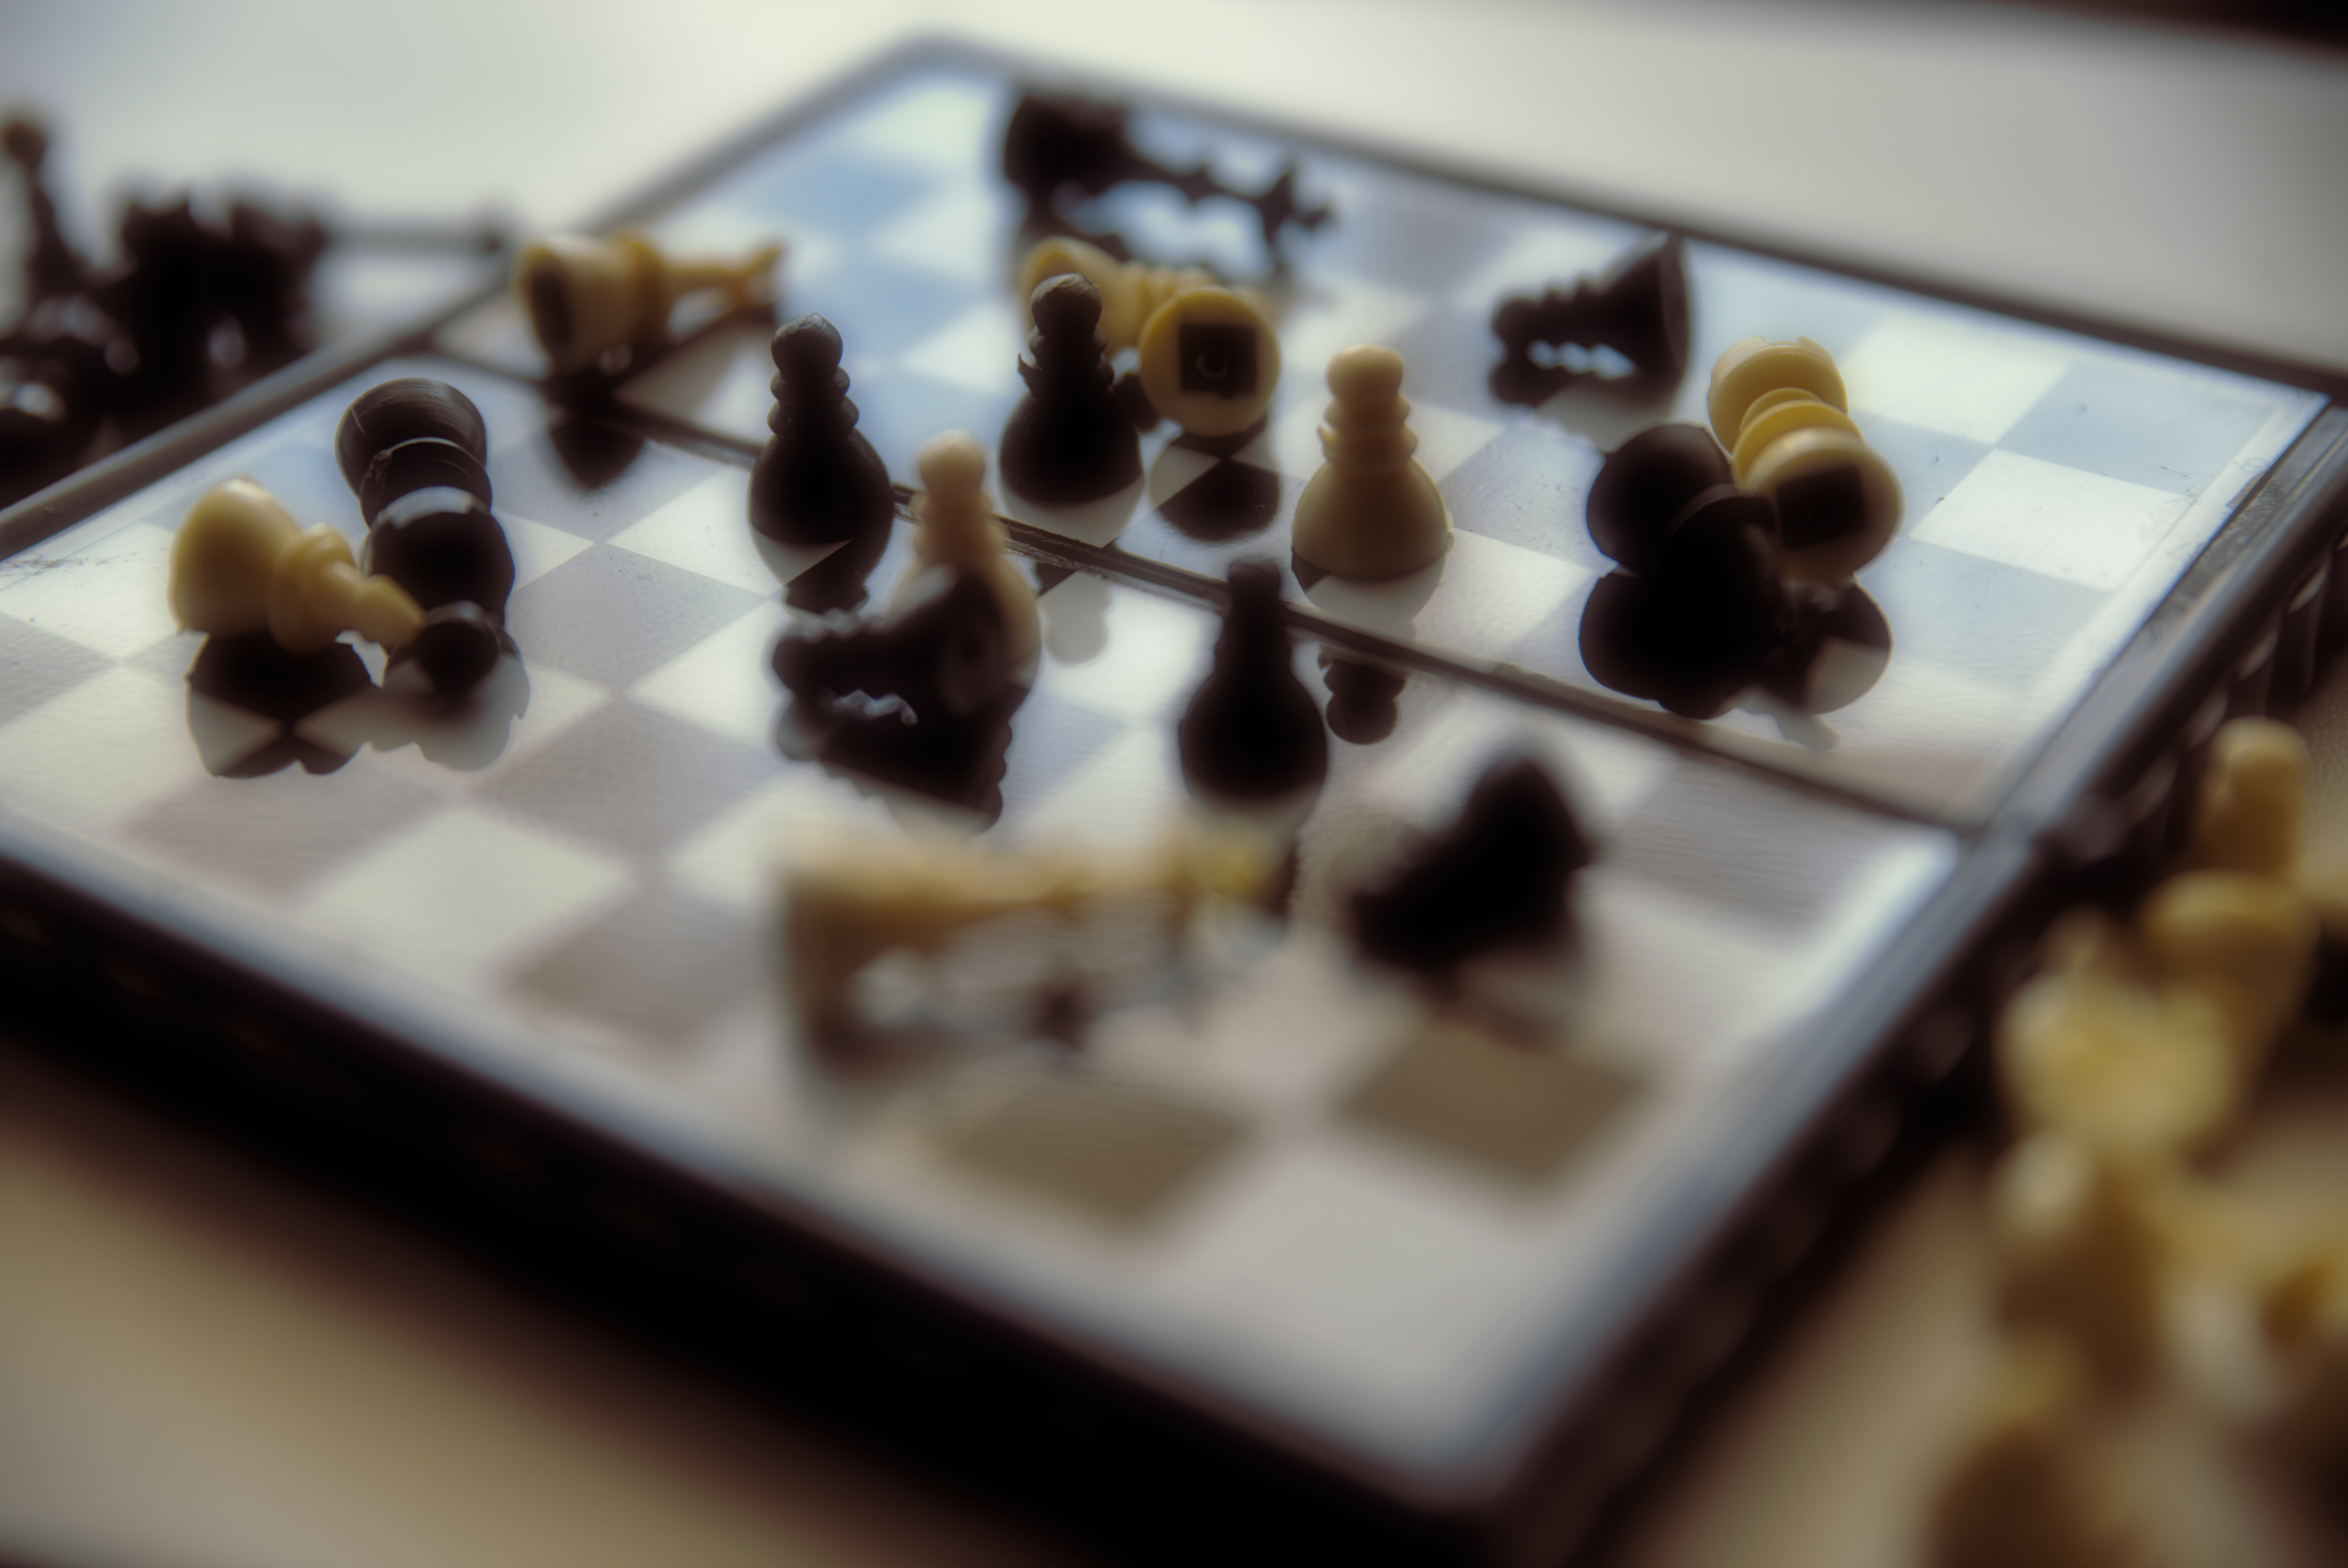
\includegraphics[width=0.9\textwidth, keepaspectratio=true]{../gfx/crochess.jpg} \\ [2.0cm]

    \textbf{\large{Mario Mlačak}} \\ [2.0cm]
\end{center}
\vspace{\stretch{1}}
\end{titlepage}

% Empty page
\thispagestyle{empty}
\vspace*{0.1\textheight}
\clearpage

% Dedication page
\thispagestyle{empty}
\vspace*{0.2\textheight}
\hfill{Dedicated to Miranda.}
\clearpage

% Publisher page
\thispagestyle{empty}
\vspace*{0.1\textheight}
\begin{center}
    \emph{Mario Mlačak} \\
    \textbf{Croatian chess} \\
    and other variants \\ [2.0em]

    \emph{Copyright} \\
    \copyright \hspace{0.2ex} 2009 -- 2016 Mario Mlačak \\
    \href{mailto:mmlacak@gmail.com}{mmlacak@gmail.com} \\ [2.0em]

    \emph{Legal} \\
    This book is published as Public Domain work. \\
    \href{https://en.wikipedia.org/wiki/Public\_domain}{https://en.wikipedia.org/wiki/Public\_domain} \\ [2.0em]

    \emph{Third, revised edition} \\
    \today \\
    Zagreb

    \vfill

    \LaTeXe
    \vspace{0.1\textheight}
\end{center}
\clearpage

% Inner title page
\thispagestyle{empty}
\vspace*{0.2\textheight}
\begin{center}
    \textbf{\Large{Croatian chess}} \\ [1.0em]
    \large{and other variants} \\ [1.0em]
    \small{3rd, revised edition} \\ [2.0cm]
    \vspace*{0.2\textheight}

    \textbf{\large{Mario Mlačak}} \\ [1.0em]
    \small{\today} % \\ [2.0cm]
\end{center}
\clearpage

% Empty page
\thispagestyle{empty}
\vspace*{0.1\textheight}
\clearpage

% Gratitude page
\thispagestyle{empty}
\vspace*{0.2\textheight}
\hfill{My most sincere gratitude to:}
\vspace*{1.0em}

\hfill{Valentina Štefanić} \\
\hspace*{\fill}{Kristina Mlačak} \\
\hspace*{\fill}{Slavko Štefanić}
\vspace*{1.0em}

\hfill{and many, many others.}
\vspace*{1.0em}

\hfill{Thank you all.}
\clearpage

% Empty page
\thispagestyle{empty}
\vspace*{0.1\textheight}
\clearpage

% Introduction page
\chapter*{Introduction}
\addcontentsline{toc}{chapter}{Introduction}

\emph{Life's too short for chess. \\
... Henry James}
\vspace*{1.0em}

I was in my aunt's house, on the border of a small village.
Through window walled garden and small brook was visible just
behind the house. And hills in the distance. Early afternoon Sun
was casting its orange rays into warm room. It was cold outside.

My cousin approached me with some nifty gizmo. He was a
few years older then me and was already going to school. \\
"Here, look at what I got." \\
"What's that?" \\
"Chess set. Wanna try? Lemme show you." \\
"Sure."

It was small plasticky, fiddly thing designed to fit into winter's
coat pocket, to be used on the go. Folding board was also used to
hold all pieces in it. Each piece was as small as humanely usable.
Each field had a hole in the middle. Bellow each piece there was
small rod fitting into those holes. It was colored all in red and ivory.

Short lesson revealed it's not that difficult to grasp what's going
on. Within minutes I picked it up. First match was, predictably, a
complete disaster. On the second go my cousin forgot about a piece,
and I grabbed his Queen gleefully. He surrendered.

After he left me with a new widget, I was intrigued. I wasn't
about playing the game, though. I was more into redesign it. Could it
be made better, more challenging, or just different? \\
'Why not make Knight jump longer, say 3 by 1 fields?' \\
'Hmmmm...' \\
'Nah, that would make jump too long for such a small board.'

Outside, the Sun was shining red.
\clearpage

% Prerequisites page
\chapter*{Prerequisites}
\addcontentsline{toc}{chapter}{Prerequisites}

\hspace{1.5em} This document describes new variants of chess, new pieces
and rules. In this document I'll describe only even variants, since
generating odd ones from there is an exercise in simplicity. Please,
see 'Even variant', 'Odd variant' in the Definitions bellow.

\textbf{\huge{TODO :: FIX ME !!!}} % TODO :: FIX ME !!!

In this document I'm assuming you have the complete prior
knowledge of classical chess pieces and rules. If not, please visit
Wikipedia entry on this subject at: \\
\href{http://en.wikipedia.org/wiki/Chess\_rules}{http://en.wikipedia.org/wiki/Chess\_rules}.
\clearpage

% Classical Game page
\chapter*{Classical Game}
\addcontentsline{toc}{chapter}{Classical Game}

\emph{A great war leaves the country with three armies - an army of
cripples, an army of mourners, and an army of thieves. \\
... German proverb}
\vspace*{1.0em}

About classical chess is written really everything already, and I
have nothing to add. Except for illustration of initial setup, so that
you can accustom yourself with rendition of pieces used in this text.

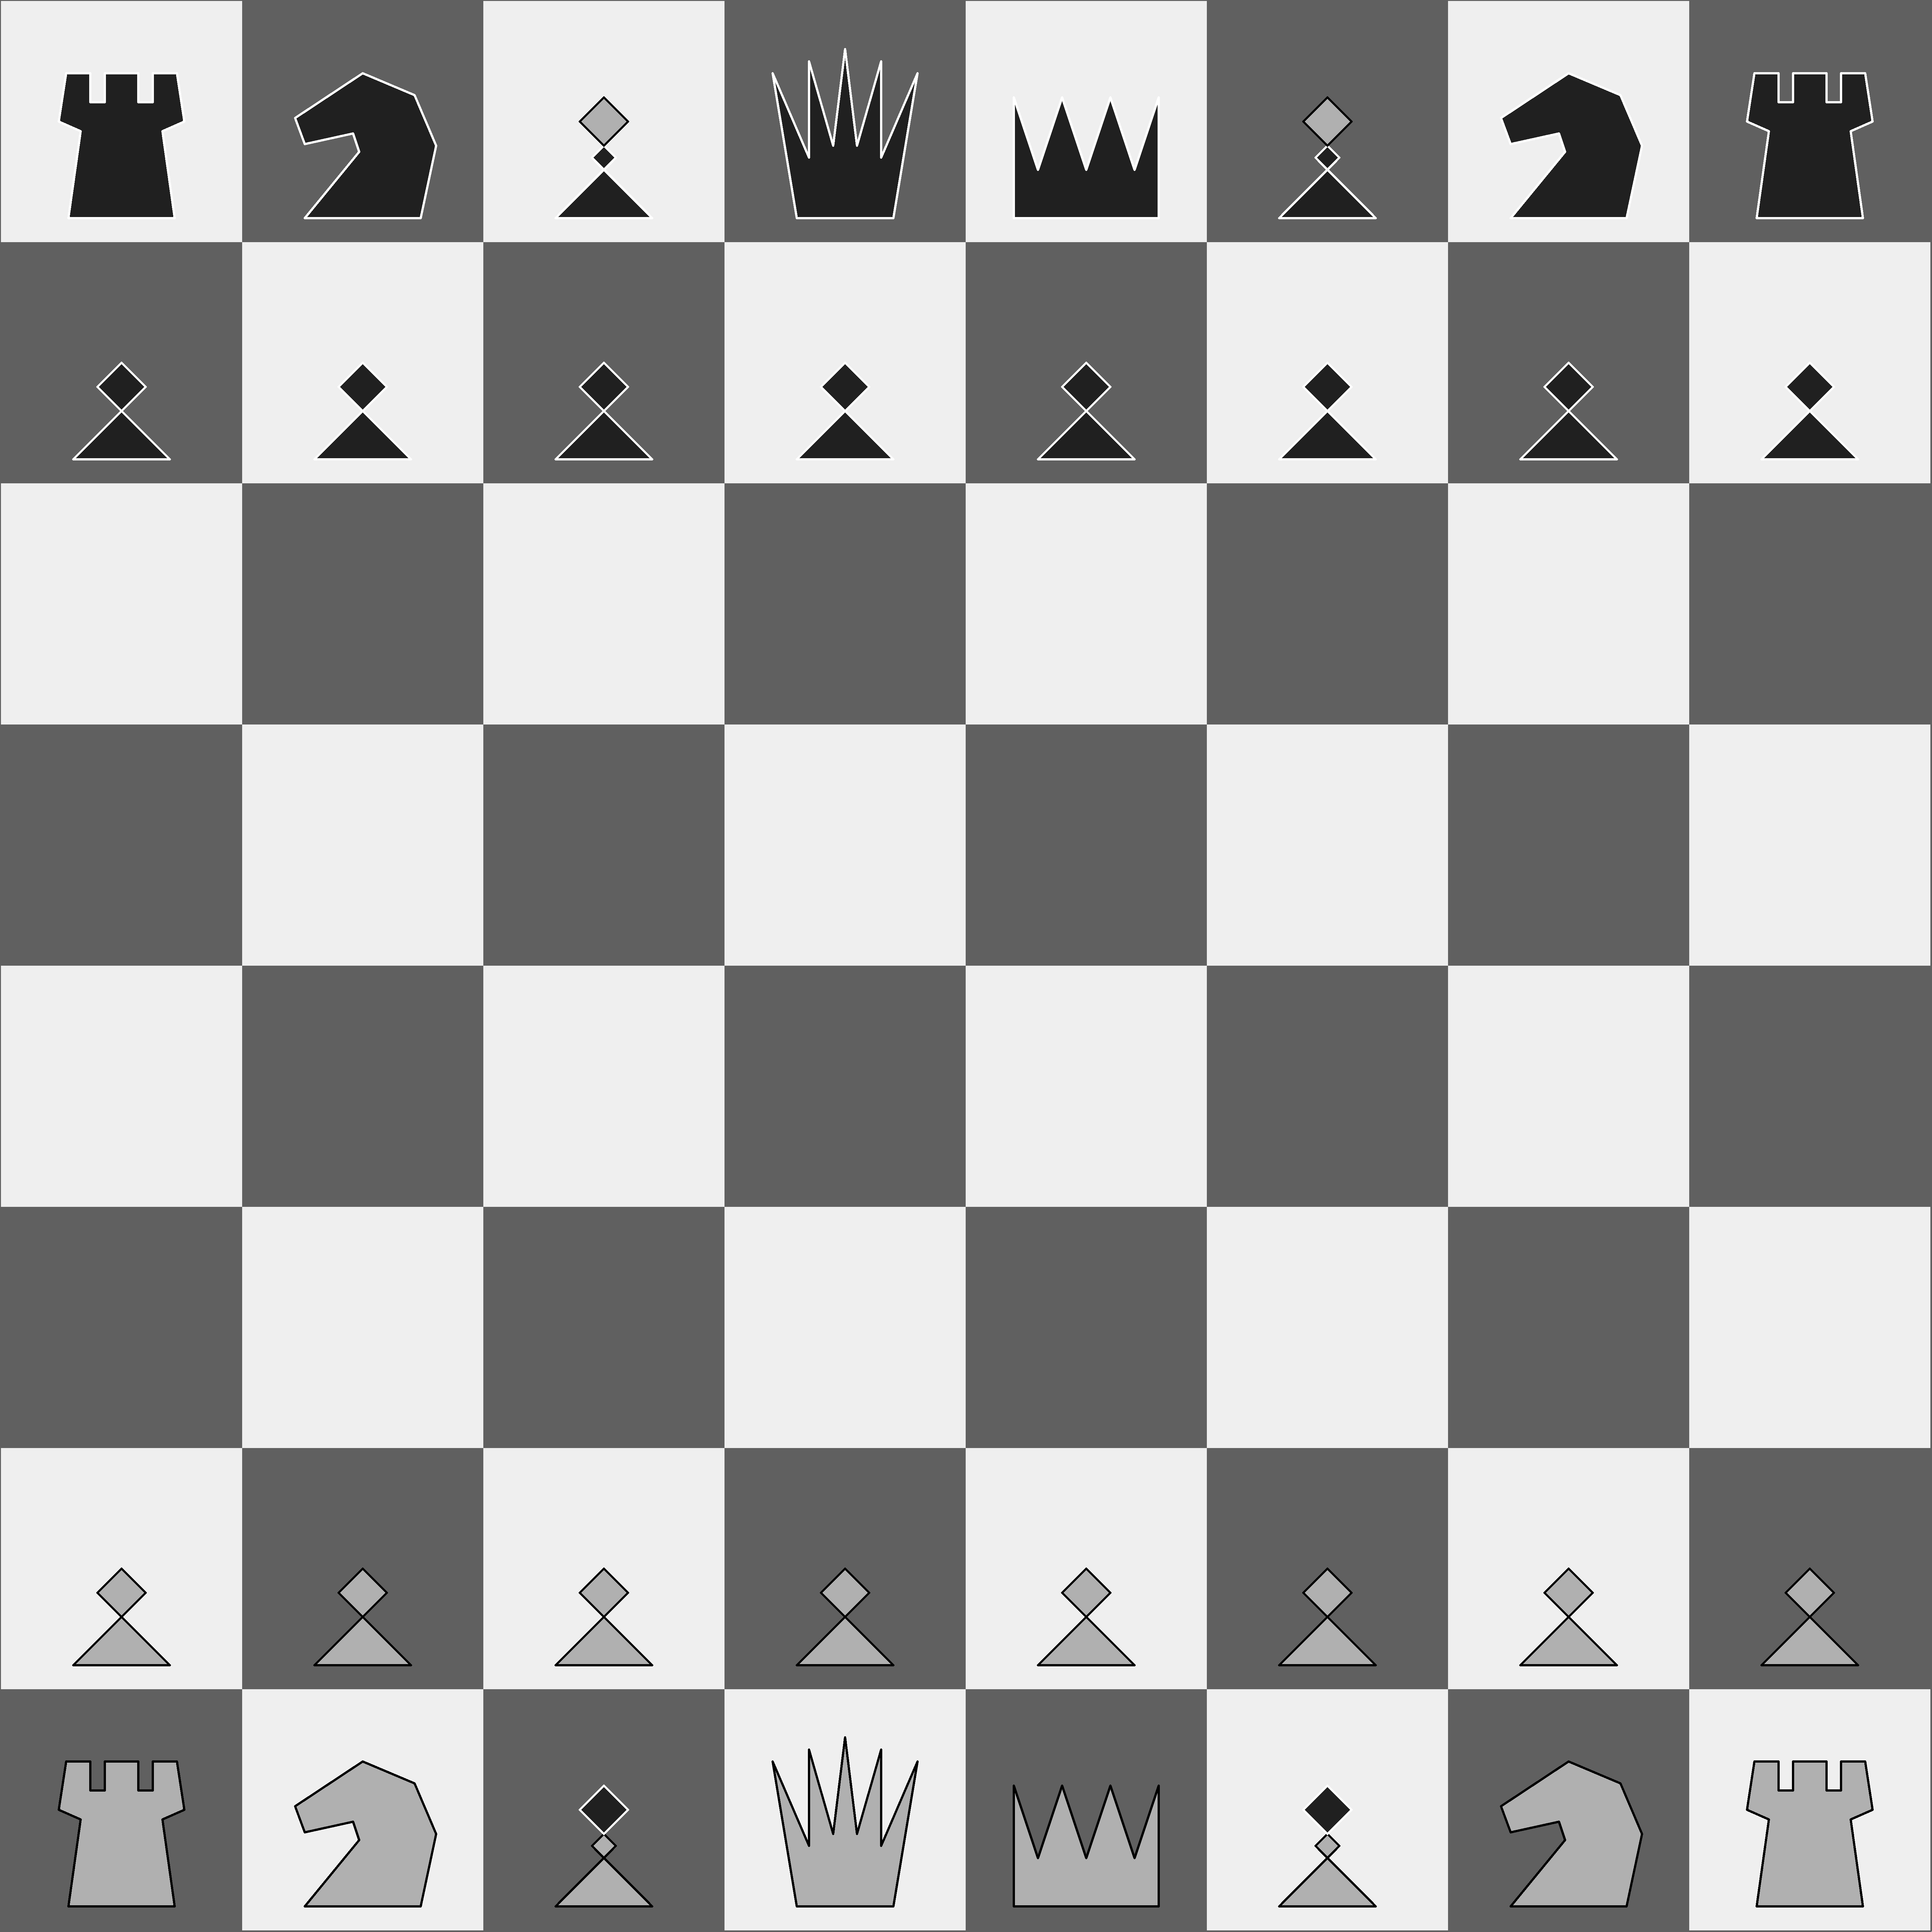
\includegraphics[width=1.0\textwidth, keepaspectratio=true]{../gfx/boards/02_classical.png}

Note that in Odd Classical Game, since it's played on 7 x 7
board, there is no en-passant move. This is so because of very
small board there is no room for a Pawn to perform 2-field initial
move without, at the same time, preventing opponent to do the same
at the same file.

\clearpage

\section*{Structure}
\addcontentsline{toc}{section}{Title of the section}
\small{This section's content... \\
abcdefghijklmnopqrstuvwxyz \\
ABCDEFGHIJKLMNOPQRSTUVWXYZ \\
0123456789}

\tiny{This section's content... \\
abcdefghijklmnopqrstuvwxyz \\
ABCDEFGHIJKLMNOPQRSTUVWXYZ \\
0123456789}

\normalsize{This section's content... \\
abcdefghijklmnopqrstuvwxyz \\
ABCDEFGHIJKLMNOPQRSTUVWXYZ \\
0123456789}

% Empty, enumerated page
\vspace*{0.1\textheight}
\clearpage

% List of figures
\listoffigures

% List of tables
\listoftables

% Table of contents
\tableofcontents
\clearpage

% % Empty page
% \thispagestyle{empty}
% \vspace*{0.1\textheight}
% \clearpage

% Challenge, end cover page
\thispagestyle{empty}
\begin{quotation}
    \it
    No FPS and racing sim [is a real challenge]. That is for
    dummies. This will make players of the game into new
    super-geniuses. Challenge to the max[imum] ... how much
    combinations there are in that [last variant] with
    teleportation, unicorn, pyramid, winged horse [Pegasus]
    and wave. How much more challenging it is compared to
    classic [chess]. Just Croatian [Ties] doubled number of
    possible combinations ...
\end{quotation}
\hspace*{\fill}{\textbf{Slavko Štefanić} [via e-mail]}
\vfill
\hspace*{\fill}{\LaTeXe}
\clearpage

\end{document}
